\documentclass[svgnames,handout,aspectratio=169]{beamer}
%\documentclass[svgnames]{beamer}

%\usepackage{natbib}
%\bibliographystyle{apalike}

\usepackage[alf]{abntex2cite}

\usepackage[utf8]{inputenc}
\usepackage[T1]{fontenc}
\usepackage{lmodern,textcomp}
%\usefonttheme{serif}
\usepackage{booktabs}
\usepackage{pict2e}[2009/06/01]
\usepackage{etoolbox}
\usepackage[brazil]{babel}
\usepackage{graphicx}
\usepackage{amsmath,amssymb,array}
\usepackage{listings}
\usepackage[all]{xy}
\usepackage{amsfonts}

\newtheorem{defi}{Definição}[section]
\newtheorem{obs}{Observação}[section]
\newtheorem{coro}{Corolário}[section]
\newtheorem{teo}{Teorema}[section]
\newtheorem{prop}{Proposição}[section]
\newtheorem{prova}{Prova}[teo]
\newtheorem{lema}{Lema}[teo]
\newtheorem{ex}{Exemplo}[section]
\newtheorem{apl}{Aplicação}[section]

%\definecolor{links}{HTML}{2A1B81}
%\hypersetup{colorlinks,linkcolor=,urlcolor=links}
%\hypersetup{colorlinks,linkcolor=links,urlcolor=links}

\graphicspath{{./figuras/}}
%\input{config}

\usetheme{default}

\setbeamertemplate{background}{
\includegraphics[width=\paperwidth,height=\paperheight]{fundo1.png}}

\setbeamertemplate{title page}{

%\includegraphics[width=\linewidth]{selimatopo.png}

\begin{center}

\vfill

\Large \textbf{{\inserttitle}}

\vfill

\textbf{Autores:}

\normalsize
\insertauthor

\end{center}

\vspace{0.3cm}

}

\setbeamercolor{frametitle}{fg=black}

\title{Escreva aqui o título do seu trabalho}

\author{
Nome Completo do Autor 1 \qquad Nome Completo do Autor 2\\
Nome Completo do Autor 3 \qquad Nome Completo do Autor 4\\
}
\date{}


\begin{document}

\begin{frame}
\maketitle
\end{frame}

\setbeamertemplate{background}{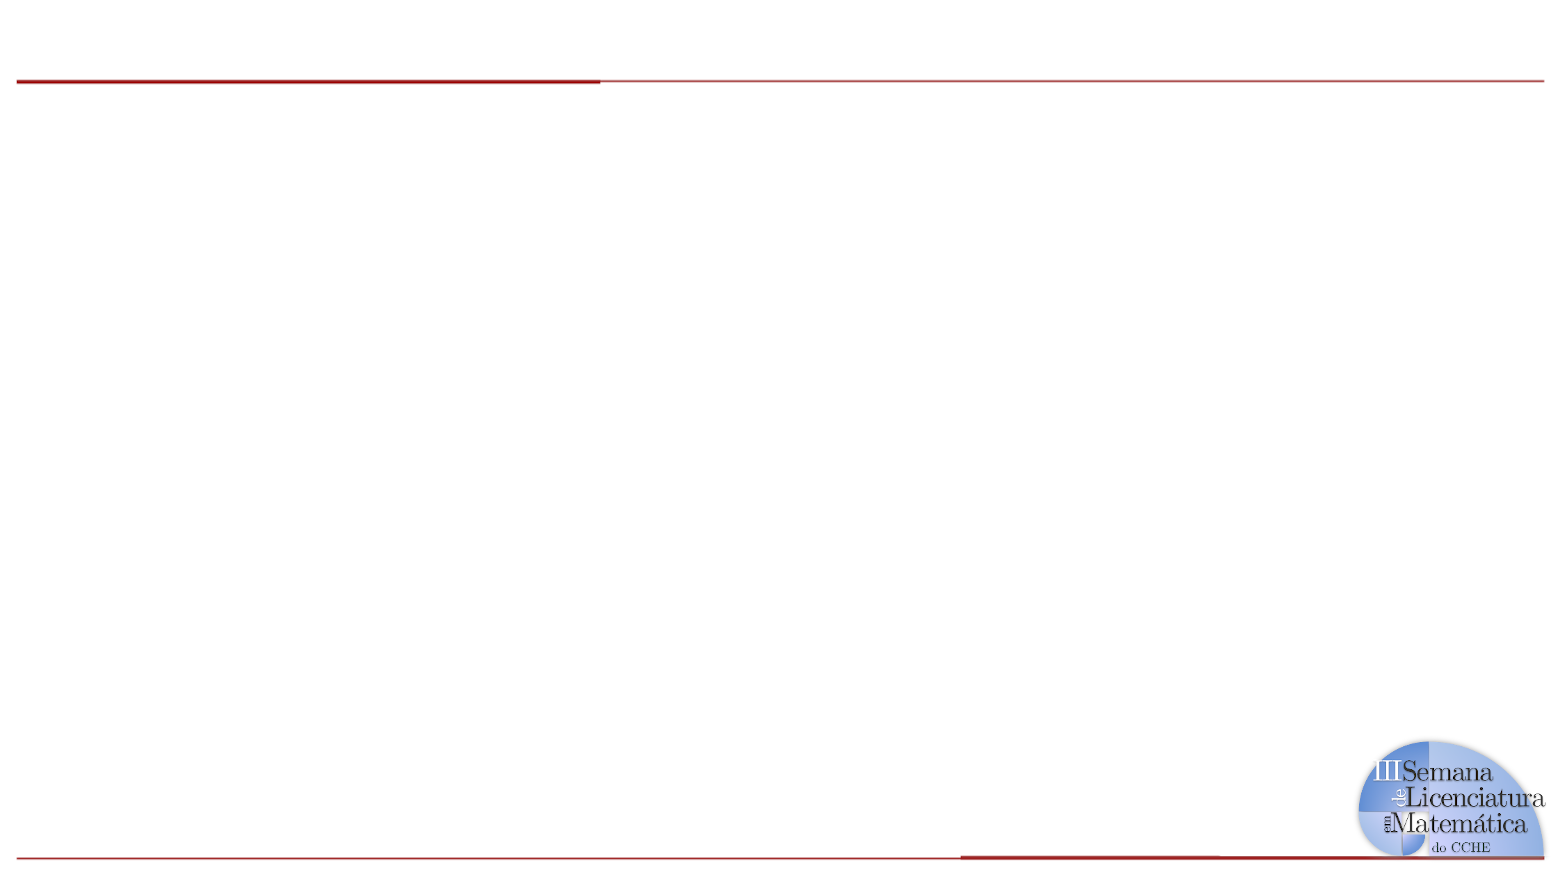
\includegraphics[width=\paperwidth,height=\paperheight,keepaspectratio]{fundo2.png}}



%Slides começam a seguir



\begin{frame}{Introdução}
\begin{itemize}
    \item O movimento de projéteis vem sendo estudado desde da antiguidade \cite{Gilat:09};
    \item Segundo \citeonline{Gilat:09}, o movimento de projéteis vem sendo estudado desde da antiguidade;    
\end{itemize}
\end{frame}





\begin{frame}{Objetivos}

\begin{itemize}
\item Desenvolver um programa de computador capaz de ser utilizado para simulações de problemas de lançamento de projéteis; 
\end{itemize}

\end{frame}




\begin{frame}{Metodologia}
\begin{itemize}
    \item Este estudo se enquadra como pesquisa aplicada, uma vez que visa investigar a aplicação de um software no ensino de funções matemáticas.
\end{itemize}
\end{frame}





\begin{frame}{Metodologia}

\textbf{Atividade 1}: o aluno deve deslizar o ponto A para as coordenadas pedidas.

\begin{figure}
    \centering
    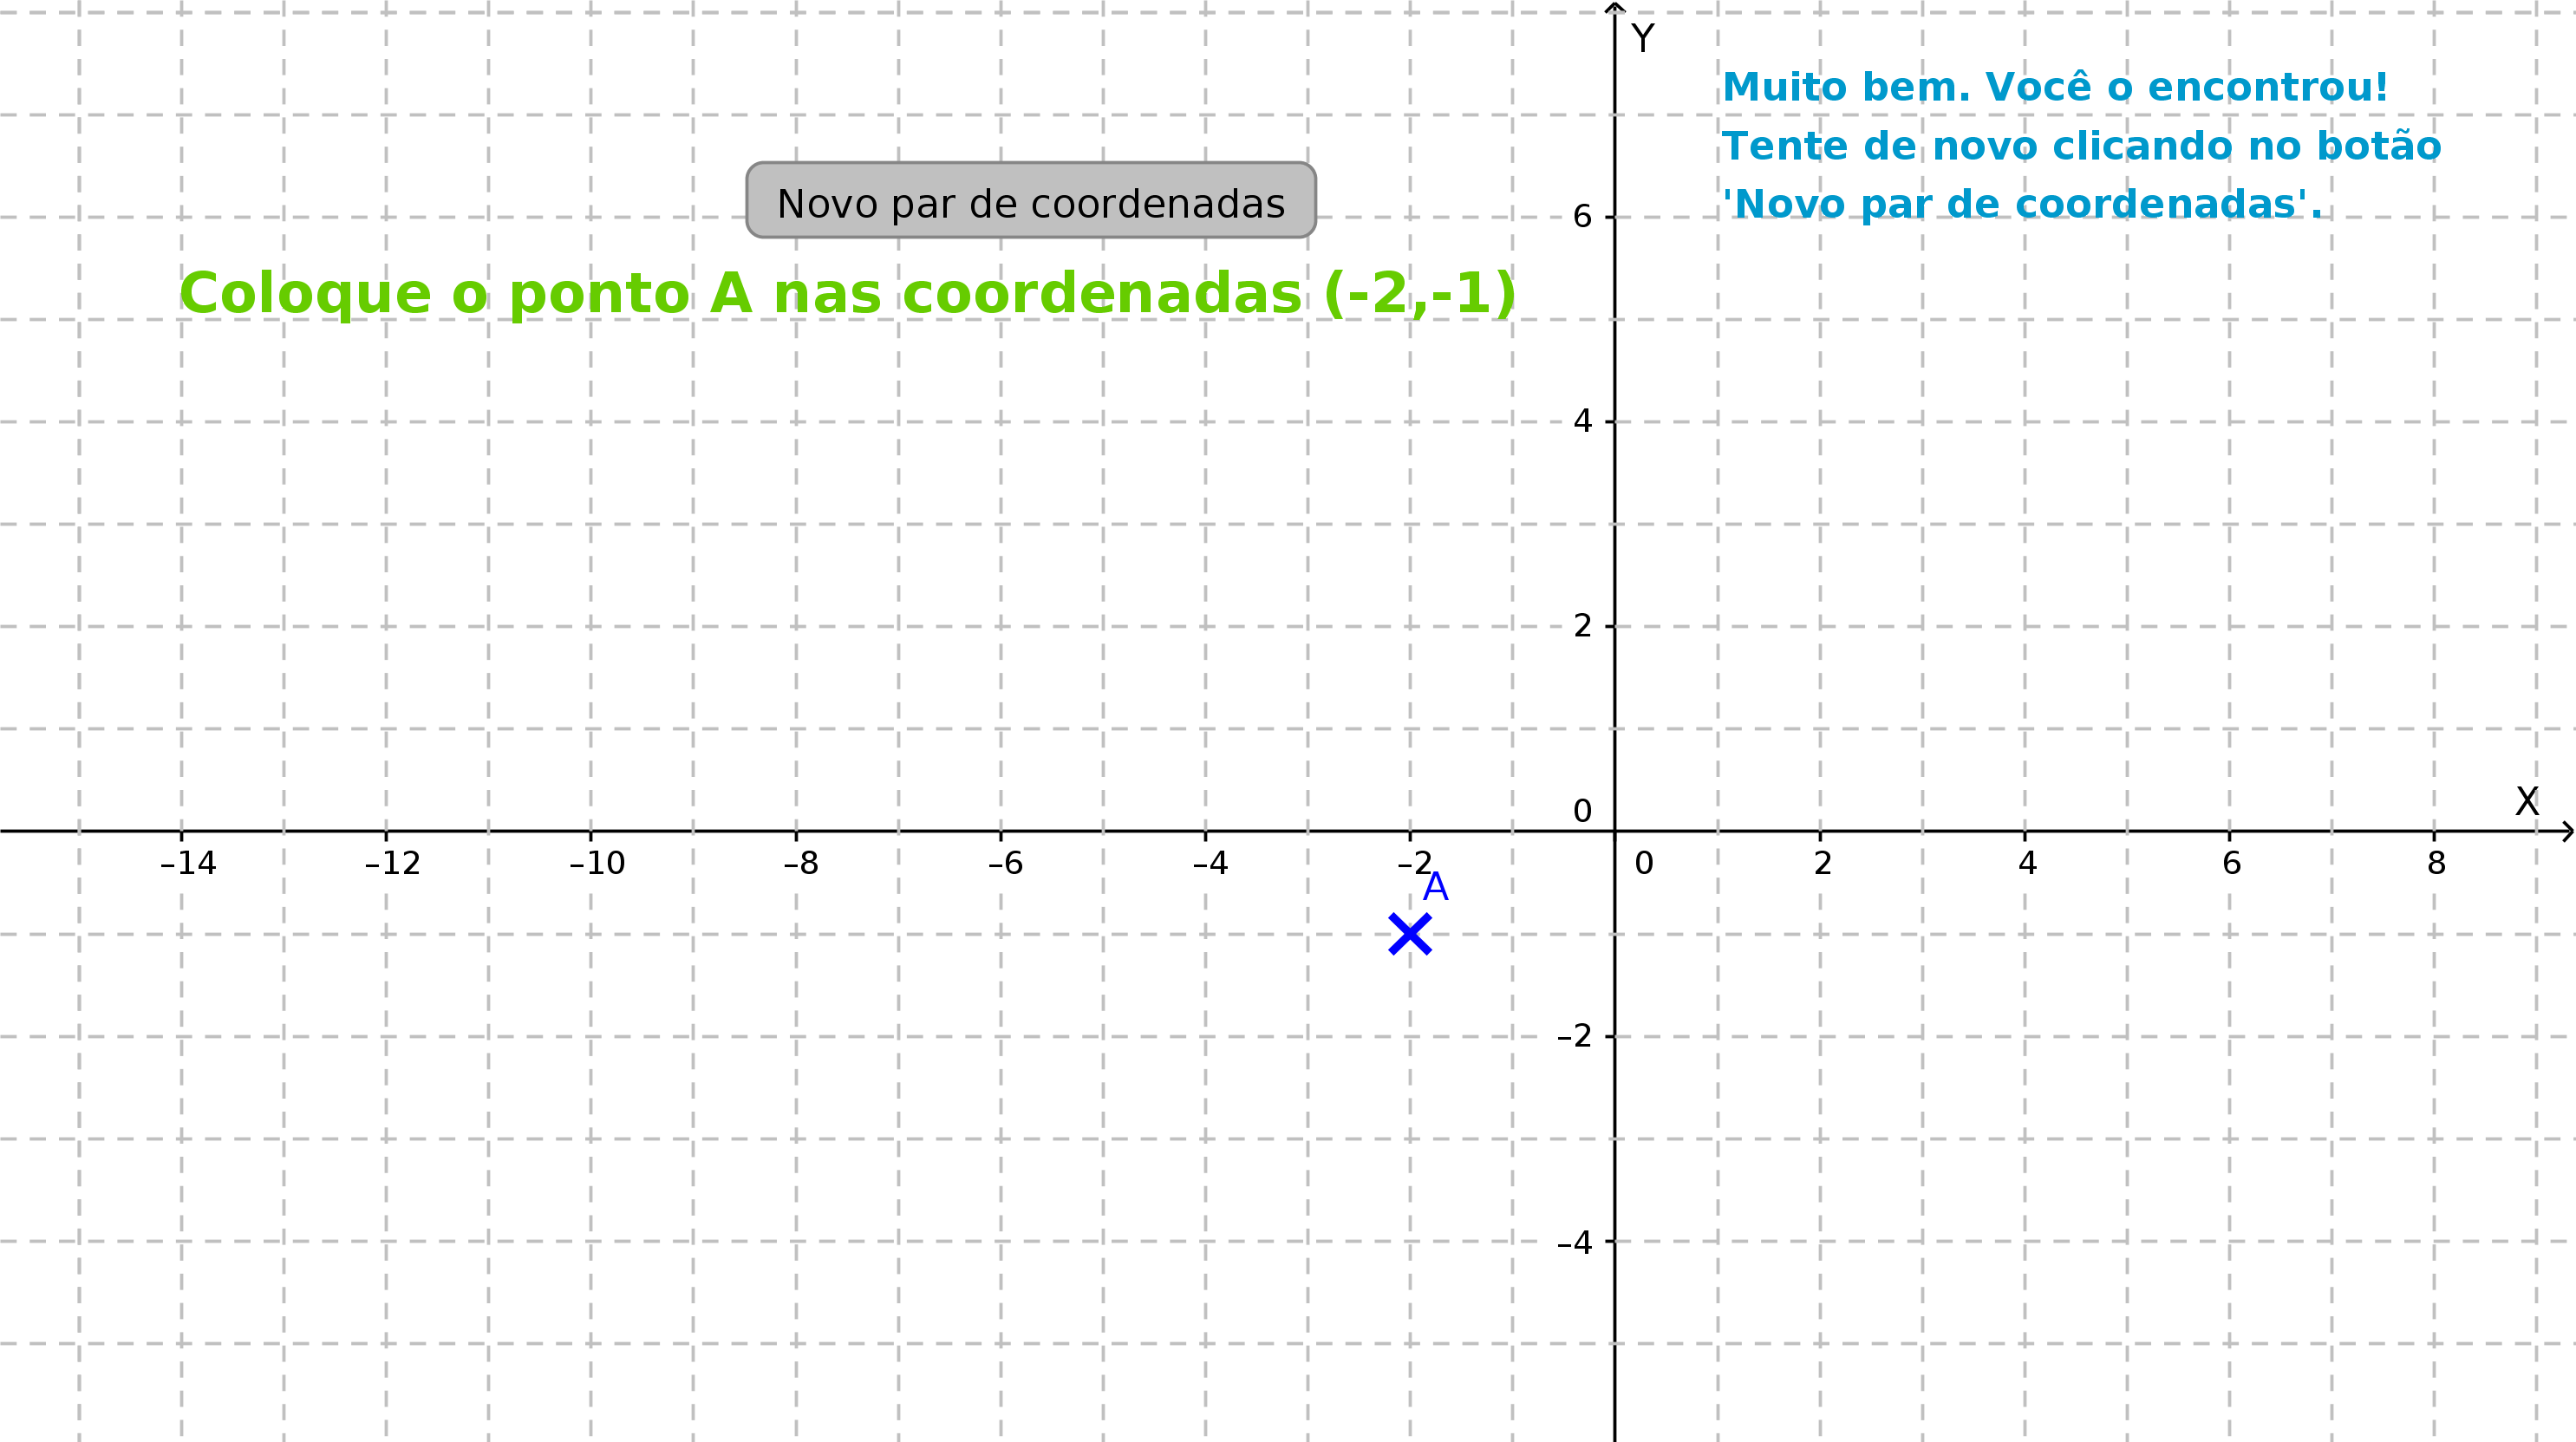
\includegraphics[width=1\linewidth]{atividade1.png} 
\end{figure}

\end{frame}




\begin{frame}{Metodologia}

A atividade visou demonstrar a influência de cada coeficiente no gráfico da função.

\begin{equation}
    f(x) = ax^2 + bx + c
\end{equation}

\begin{equation}
    \Delta = b^2-4ac
\end{equation}

\begin{equation}
    y_v = \frac{-\Delta}{4a}
\end{equation}

\begin{equation}
    x_v = \frac{-b}{2a}
\end{equation}

\begin{equation}
    x = \frac{-b \pm \sqrt{\Delta}}{2a}
\end{equation}
\end{frame}





\begin{frame}{Resultados e discussão}

\begin{itemize}
    \item Questionário aplicado ao final dos encontros:
\begin{enumerate}
    \item Qual a diferença entre uma aula tradicional, ou seja, com o quadro negro, e exposição com o software GeoGebra?
\end{enumerate}
\end{itemize}
\end{frame}





\begin{frame}{Conclusão}

\begin{itemize}
    \item Os softwares educacionais se tornaram ótimas alternativas de apoio às atividades em sala de aula;
\end{itemize}
\end{frame}





\begin{frame}{Referências}
\bibliography{references}

\end{frame}





%\begin{frame}{Obrigado!}
%        
\includegraphics[width=5cm]{Marca-da-UEPB.png}\hspace{2.8cm}
\includegraphics[width=3.cm]{cche.png}
%\end{frame}






\end{document}


